%%
%% Skript Differentialgeometrie im Wintersemester 12/13
%% Zur Vorlesung von Dr. Grensing am KIT Karlsruhe
%%
%% Uebung 1
%%

\section{29. Oktober 2012}
\setcounter{Aufg}{0} %Damit die Aufgaben jedes Mal bei Aufgabe 1 anfangen
\setcounter{Loes}{0}

\begin{Loes}\ \\
\begin{center}\begin{tikzpicture}[font=\scriptsize]
	%\draw[step=0.25,gray!15] (-3,-3) grid (3,3); \draw[step=0.5,gray!30] (-3,-3) grid (3,3); %\fill (0,0) circle(0.1); %Hilfsgitter
	\def\radius{1.5}
	\def\smallLength{2.75}
	\def\biglength{3.75}
	\def\height{0.75}
	\def\angle{25}
	
	\path[name path=circle,draw] (0,0) circle (\radius);
	\begin{scope}
			\clip (-\radius - 0.25,0) rectangle (\radius + 0.25,-\radius - 0.25);
			\draw (0,0) ellipse (1.5 and 0.5);
		\end{scope}\begin{scope}
			\clip (-\radius - 0.25,0) rectangle (\radius + 0.25,\radius + 0.25);
			\draw[dashed] (0,0) ellipse (1.5 and 0.5);
		\end{scope}
	\path[name path=vert] (\smallLength,\height) -- (-\smallLength,\height);
	\path[name intersections={of=circle and vert}];
	\draw (\biglength,-\height) -- (\smallLength,\height) -- (intersection-1) (intersection-2) -- (-\smallLength,\height) -- (-\biglength,-\height) -- (\biglength,-\height);
	\draw[dashed] (intersection-1) -- (intersection-2);
	
	\coordinate (N) at (0,\radius); \coordinate (S) at (0,-\radius); \coordinate (Pkt1) at (-2,-0.25); \coordinate (direction) at (-0.6,1.25); \coordinate (direction2) at (0.6,1.25);
	
	\path[name path=upper,draw] (N) node[above]{$N$} -- (Pkt1)node[left]{$(0,\phi(p))$}; \fill (N) circle (0.05) (Pkt1) circle (0.05);
	
	\path[name path=left] (S) node[below]{$S$} -- ($(S)+2*(direction)$); \fill (S) circle (0.05); \path[name intersections={of=upper and left}];
	\draw (intersection-1) node[right]{$p$} -- (S); \fill (intersection-1) circle (0.05); \fill ($(S)+1.1*(direction)$) circle(0.05) node[right]{$(0,\psi(p))$};
	
	\draw (S) -- ($(S)+2.5*(direction2)$); \fill ($(S)+1.25*(direction2)$) circle(0.05) node[right]{$(0, \phi(p))$};
\end{tikzpicture}\end{center}
\begin{enumerate}[label=\alph*),leftmargin=*,widest=a,font=\normalfont]
\item
	$S^n = (S^n \setminus \{N\}) \cup (S^n\setminus \{S\}) \checkmark$
	
	$\phi, \psi$ Hom"oomorphismen, $\Phi: \{(x^0,\ldots ,x^n) \in \R^n | x^0 < 1\} \to \R^n, x \mapsto \frac{1}{1-x^0}(x^1, \ldots ,x^n) \Rightarrow \Phi$ ist stetig $\Rightarrow  \phi = \Phi|_{S^n \setminus \{N\}}$ ist stetig. Es ist
		\[ \phi^{-1}(y) = \frac{1}{1+|y|^2}(\|y\|^2 - 1, 2y)\]
	also ist $\phi^{-1}$ stetig. Analog f"ur $\psi$:
		\[\phi \circ \psi^{-1}(y) = \frac{y}{\|y\|^2} = \psi \circ \phi{-1}(y) \]
	f"ur $y \in \R^n \setminus \{0\}$. Also glatter Kartenwechsel.\marginnote{\begin{tikzpicture}[font=\scriptsize]
		\def\radius{1.25}
		\def\angle{22}
		\def\anglePoint{65}	
		\path[name path=circle,draw] (0,0) circle (\radius);
		\begin{scope}
			\clip (-\radius - 0.25,0) rectangle (\radius + 0.25,-\radius - 0.25);
			\draw (0,0) ellipse (1.25 and 0.25);
		\end{scope}\begin{scope}
			\clip (-\radius - 0.25,0) rectangle (\radius + 0.25,\radius + 0.25);
			\draw[dashed] (0,0) ellipse (1.25 and 0.25);
		\end{scope}
		\draw[->] (\anglePoint:\radius) node[anchor=south west]{$p$} -- ($(\anglePoint:\radius)+(270:1.2)$); \fill (\anglePoint:\radius) circle(0.05) ($(\anglePoint:\radius)+(270:1.25)$) circle(0.05) node[anchor=north]{$\phi_i^+(p)$};
	\end{tikzpicture}}
		\[ \phi_i^\pm: U_i^\pm \to B_1(0) \subset \R^n, x \mapsto (x^0,\ldots ,x^{i-1}, x^{i+1},\ldots ,x^n) \]
		\[ (\phi_i^\pm)^{-1}: B_1(0) \to U_i^\pm, y \mapsto (y^0,\ldots ,y^{i-1}, \pm (1 - \|y\|^2), \textcolor{red}{y^i},\ldots ,y^{n+1}) \]
	$\phi_i^\pm \circ (\phi_j^\pm)^{-1}$ glatt
	
	$\psi \circ (\phi_j^\pm)^{-1}$ glatt
	
	$\phi \circ (\phi_j^\pm)^{-1}$ glatt
	
	$\phi_i^\pm \circ \phi$ glatt
	
	$\phi_i^\pm \circ \psi$ glatt
\item
	asdf
\end{enumerate}
\end{Loes}

\begin{Loes}
$\phi: \R \to \R, x \mapsto x^3$

\emph{Behauptung:} $\phi$ induziert eine $C^\infty$-Struktur auf $\R$, die von der Standardstruktur abweicht.

Dazu m"ussen wir zeigen:\begin{enumerate}[font=\normalfont,label=(\roman*)]
\item
	$\{(\phi, \R)\}$ ist ein $C^\infty$-Atlas
\item
	$\phi$ ist nicht vertr"aglich mit $(\Id, \R)$
\end{enumerate}
\emph{Beweis:}\begin{enumerate}[leftmargin=*,widest=ii,font=\normalfont,label=(\roman*)]
\item
	$\phi$ ist Hom"oomorphismus, da $\phi$ und $\phi^{-1}: x \mapsto \sqrt[3]{x}$ stetig sind. Offensichtlich "uberdeckt $\phi$ ganz $\R$. Der einzige Kartenwechsel $\phi \circ \phi^{-1} = \Id_{\R}$ ist glatt.
\item
	Betrachte
		\[ \Id_{\R} \circ \phi^{-1} = \phi^{-1}: x \mapsto \sqrt[3]{x} \]
	$\Id_{\R} \circ \phi^{-1}$ ist in $0$ nicht differenzierbar $\Rightarrow$ (ii) $\checkmark$
\end{enumerate}
\begin{description}[font=\normalfont\itshape]
\item[Behauptung:]
	Die beiden $C^\infty$ Strukturen sind diffeomorph
\item[Beweis:]
	Sei
		\[\begin{array}{cccc} f:&  \overset{\text{von } \Id \text{ induziert}}{(\R, \tau_{\text{std}})} &\to& \overset{\text{von } \phi \text{ induziert}}{(\R, \tau)} \\
			& x &\mapsto& \sqrt[3]{x} \end{array}\]
	\marginnote{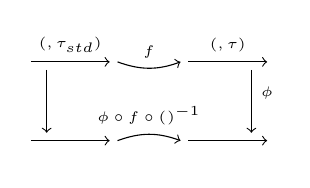
\begin{tikzpicture}[font=\tiny]
	\draw[->] (-1.5,0.5) -- node[above]{$(\R,\tau_{\text{std}})$} (-0.5,0.5); \draw[->] (0.5,0.5) -- node[above]{$(\R,\tau)$} (1.5,0.5);
	\draw[->] (-1.5,-0.5) -- node[below]{$\R$} (-0.5,-0.5); \draw[->] (0.5,-0.5) -- node[below]{$\R$} (1.5,-0.5);
	\draw[->] (-1.3,0.4) --node[left,yshift=3]{$\Id$} (-1.3,-0.4); \draw[->] (1.3,0.4) --node[right,yshift=3]{$\phi$} (1.3,-0.4);
	\draw[->] (-0.4, 0.5) to[out=340,in=200]node[above]{$f$} (0.4,0.5); \draw[->] (-0.4, -0.5) to[out=20,in=160]node[above]{$\phi \circ f \circ (\Id_{\R})^{-1}$} (0.4,-0.5);
	\end{tikzpicture}}
	Dann ist $f$ bijektiv. Es gilt f"ur $x \in \R$:
		\[ \phi \circ f \circ (\Id_{\R})^{-1} (x) = (\sqrt[3]{x})^3 = x \]
	ist glatt. Betrachte nun $f^{-1}$: $\Id_{\R} \circ f^{-1} \circ \phi^{-1}(x) = (\sqrt[3]{x})^3 = x$ ist glatt. Damit ist $f$ ein Diffeomorphismus.
\end{description}
\end{Loes}

\begin{Loes}
$k \in \N \cup \{\infty\}$, $M_1, M_2$ $C^k$-Mannigfaltigkeiten, $N_i \subseteq M_i$ Untermannigfaltigkeit, $f \in C^j(M_1, M_2)$ wobei $j \le k$, $f(N_1) \subseteq N_2$.
\begin{description}[font=\normalfont\itshape]
\item[Behauptung:]
	$f|_{N_1} \in C^j(N_1, N_2)$
\item[Beweis:]
	Sei $p \in N_1$, sei $(\phi_1, U_1)$ eine adoptierte Karte von $M_1$ in $p$, das hei\ss t $p \in U_1$.
		\[ \phi_1(U_1 \cap N_1) = \phi_1(U_1) \cap \left(\R^{\dim N_1} \times \{0\}^{n-\dim N}\right) \]
	Sei $(\phi_2, U_2)$ eine adoptiere Karte von $N_2$ um $f(p)$. Dann erhaltenen wir Karten von $N_i$, indem wir die Projektion $\pi_i: \R^{\dim M_i} \to \R^{\dim N_i}, x \mapsto (x^1,\ldots ,x^{\dim N_i})$ hinter die Karten $\phi_i$ schalten (das hei\ss t betrachte $\pi_i \circ \phi_i$).
	
	Es ist
		\[(\pi_2 \circ \phi_2) \circ f|_{N_1} \circ (\pi_1 \circ \phi_1)^{-1} = \underbrace{\pi_2}_{C^\infty} \circ (\underbrace{\phi_2 \circ f \circ \phi_1^{-1}}_{C^j}) \circ C_1\]
	mit $C_1: \R^{\dim N_1} \ni x \mapsto (x, 0,\ldots ,0) \in \R^{\dim M_1}$. Also $(\pi_2 \circ \phi_2) \circ f \circ (\pi_1 \circ \phi_1)^{-1} \in C^j$ und damit $f|_{N_1} \in C^j(N_1, N_2)$
\end{description}
\end{Loes}

\begin{Loes}\begin{enumerate}[label=\alph*),leftmargin=*,widest=a,font=\normalfont]
\item
	$M = S^n$, $N = \{(x^0, x^1, \ldots ,x^n) \in S^n | x^2 = \ldots = x^n = 0\}$; Skizze f"ur $n = 2$:
	\begin{center}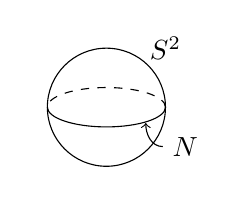
\begin{tikzpicture}
		\draw (0,0) circle (0.75);
		\begin{scope}
			\clip (-1,0) rectangle (1,-1);
			\draw (0,0) ellipse (0.75 and 0.25);
		\end{scope}\begin{scope}
			\clip (-1,0) rectangle (1,1);
			\draw[dashed] (0,0) ellipse (0.75 and 0.25);
		\end{scope}
		\node at (0.75,0.75) {$S^2$}; \node (N) at (1,-0.5) {$N$};
		\draw[->] (N) to[out=180,in=270] (0.5,-0.2);
	\end{tikzpicture}\end{center}
	\begin{description}[font=\normalfont\itshape]
	\item[Behauptung:]
		$N$ ist eine Untermannigfaltigkeit von $M$.\marginnote{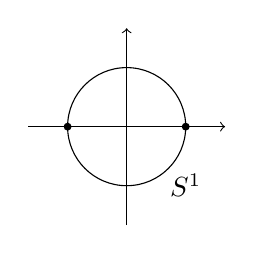
\begin{tikzpicture}
			\draw[->] (-1.25,0) -- (1.25,0); \draw[->] (0,-1.25) -- (0,1.25);
			\draw (0,0) circle (0.75); \fill (-0.75,0) circle (0.05) (0.75,0) circle (0.05); \node at (0.75,-0.75) {$S^1$};
		\end{tikzpicture}}
	\item[Beweis:]
		Sei $\phi: \overbrace{S^n \setminus \{(1, 0,\ldots ,0)\}}^{=:U} \to \R^n$, $\phi(x) = \frac{1}{1-x^0}(x^1,\ldots ,x^n)$
		
		\emph{Zu zeigen:} $\phi(U \cap N) = \phi(U) \cap (\R \times \{0\}^{n-1})$
			\[ \phi(U \cap N) = \phi(N \setminus \{(1,\ldots ,0)\}) = \R \times \{0\}^{n-1} \]
		F"ur $p \in N \setminus \{(1,0, \ldots ,0)\}$ ist $\phi$ also eine adoptierte Karte um $p$. F"ur $p = (1, 0, \ldots, 0)$ ist analog $\psi$ (aus 1 a)) eine adoptierte Karte.
	\end{description}
\item
	$M = \R^2$, $N = \{(x, 0) | x \ge 0\} \cup \{(0,y)|y \ge 0\}$; Skizze:
	\begin{center}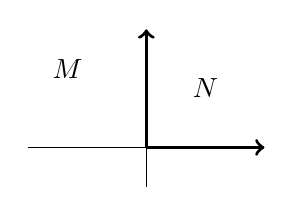
\begin{tikzpicture}
		\draw (-1.5,0) -- (0,0); \draw[very thick,->] (0,0) -- (1.5,0);
		\draw (0,-0.5) -- (0,0); \draw[very thick,->] (0,0) -- (0,1.5);
		\node at (-1,1) {$M$}; \node at (0.75,0.75) {$N$};
	\end{tikzpicture}\end{center}
	\begin{description}[font=\normalfont\itshape]
	\item[Behauptung:]
		$N$ ist keine glatte Untermannigfaltigkeit von $\R$.
	\item[Beweis:]
		Angenommen $N$ w"are Untermannigfaltigkeit von $\R^2$. Da $N$ hom"oomorph zu $\R$ ist, w"are es eine eindimensionale Untermannigfaltigkeit. Damit existiert eine Karte $(\phi, U)$ von $\R^2$ um $(0,0)$ mit $\phi(U\cap N) = \phi(U) \cap (\R \times \{0\})$. Betrachte $\phi^{-1}$, beziehungsweise $f(t) = \phi^{-1}(t,0)$. Es sei $t_0 \in \R$ mit $f(t_0) = (0,0)$. Da $f(t) = N \cap U$ ist entweder $f(t) \in \{(0, y) | y \ge 0\}$ f"ur $t > t_0$ und $f(t) \in \{(x, 0) | x \ge 0\}$ f"ur $t < t_0$ oder umgekehrt. Dann ist $f'(t) \in \R e_2$ f"ur $ t > t_0$ und $f'(t) \in \R e_1$ f"ur $t < t_0$ oder umgekehrt.
		
		$\Rightarrow f'(0) \in \R e_1 \cap \R e_2 = \{(0,0)\}$
		
		\emph{Andererseits:} $f'(0) = \underbrace{(D \phi^{-1}|_{\phi(0,0)})}_{\text{Isom., da } \phi^{-1} \text{ Diffeom.}}(\left(\begin{smallmatrix}1\\0\end{smallmatrix}\right)) \ne \left(\begin{smallmatrix}1\\0\end{smallmatrix}\right)$
	\end{description}
\end{enumerate}\end{Loes}